% Pyrenees research update
% Robert Wright, 22 May 2022

\documentclass[english, xcolor=dvipsnames, 11pt]{beamer}

\usepackage{polyglossia}
\setmainlanguage[variant=british]{english}
\usepackage[style=british]{csquotes}
\usepackage{translator} % doesn't recognise the language set of polyglossia
\usepackage{siunitx}[=v2] % requires "translator" package 
\sisetup{%
	separate-uncertainty=true,
	locale = UK,
}
\usepackage{pgfpages}
\usepackage[absolute,overlay]{textpos}
\setlength{\TPHorizModule}{1mm}
\setlength{\TPVertModule}{1mm}
\usepackage{graphicx}
\usepackage{float}
\usepackage{booktabs}
\usepackage{mathtools}
\usepackage[center]{caption}
\usepackage{subcaption}
\usepackage[nodayofweek]{datetime} % load after language is set!
\newdate{prsnt}{22}{5}{2022}
\usepackage{hyperref}
\hypersetup{
	colorlinks=true,
	urlcolor=.,
	linkcolor=,
	citecolor=,
	%pdftitle={Overleaf Example},
}

\usepackage[%
backend=biber,
style=numeric-comp,
autolang=langname,
uniquename=init,
giveninits=true,
maxnames=2,
]{biblatex}
\renewcommand{\bibfont}{\small}
\AtEveryBibitem{
	\clearfield{url}
	\clearfield{urlyear}
}
\addbibresource{lit-butterflys.bib}

% set style
\usepackage{listings}
\usepackage{xcolor}
\usepackage{courier}
\usetheme[background=dark]{metropolis} % Themenwahl
\setbeamercolor{palette primary}{bg=PineGreen}
\setbeamercolor{alerted text}{fg=PineGreen}

% TITLE

\title{iLINKmeeting}
\subtitle{Assessing time series of daily butterfly monitoring data in the Baltic}
\author{Robert Wright}
\institute{Botanical Institute of Barcelona (IBB)}
\date{\displaydate{prsnt}}

\begin{document}
	
	\maketitle
	
	%%%%%%%%%%%%%%%%%%%%%%%%%%%%%%%%%%%%%%%%%%%%%%%%%%%%%%%%%%%%%%%%
	
	\begin{frame}{Data acquisition}
		\begin{columns}[t]
		\column{0.5\textwidth}
		\begin{figure}
			\centering
			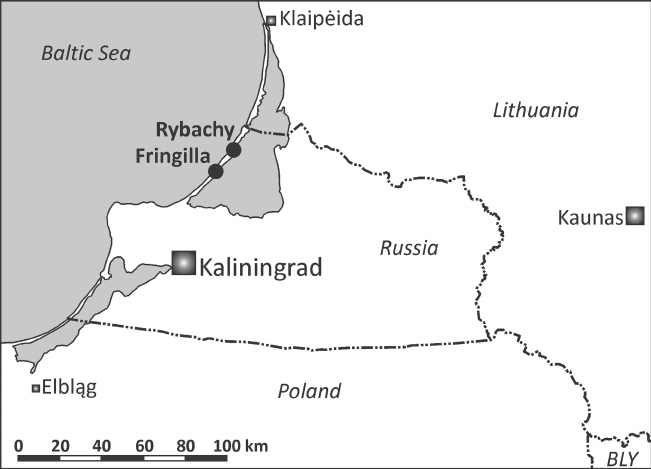
\includegraphics[width=0.9\textwidth]{figs/0-Map-of-the-Kaliningrad-Oblast-Russia-with-location-of-the-study-site-on-the-Courish.png}
			\caption{Map of Kaliningrad Oblast with location of the study site \enquote{Fringilla} on Courish Spit \parencite{shapoval2012}}
			\label{fig:site-location}
		\end{figure}
		\column{0.5\textwidth}
		\begin{figure}
			\centering
			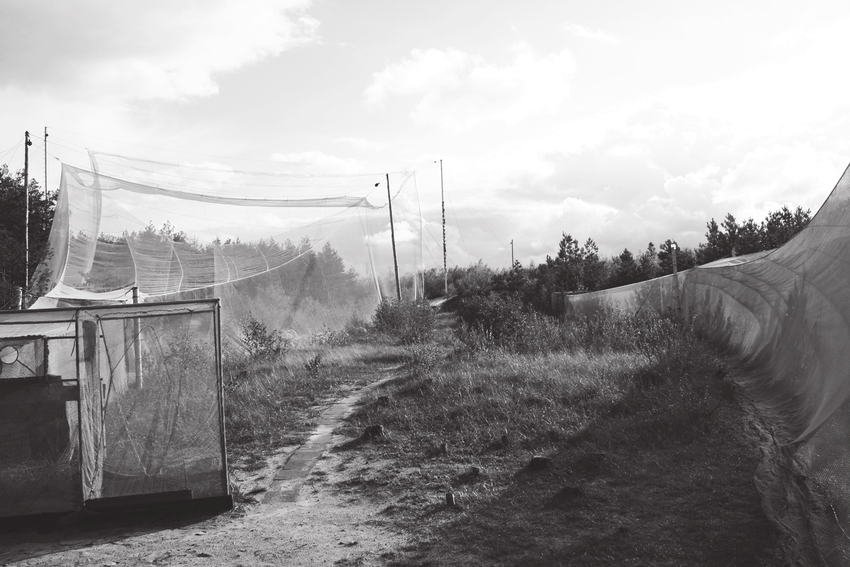
\includegraphics[width=0.9\textwidth]{figs/0-Ornithological-Rybachy-traps-on-the-Courish-Spit-Biological-Station-Fringilla-near.png}
			\caption{Ornithological \enquote{Rybachy} traps on Courish Spit \parencite{shapoval2012}}
			\label{fig:traps}
		\end{figure}
		\end{columns}
		\begin{itemize}
			\item[\(\rightarrow\)] collected by \textbf{Anatoly Shapoval} \& \textbf{Nazar Shapoval}, Russian Academy of Sciences
		\end{itemize}
	\end{frame}
		
	%%%%%%%%%%%%%%%%%%%%%%%%%%%%%%%%%%%%%%%%%%%%%%%%%%%%%%%%%%%%%%%%
	
	\begin{frame}{Preliminary analysis}
		\begin{figure}
			\centering
			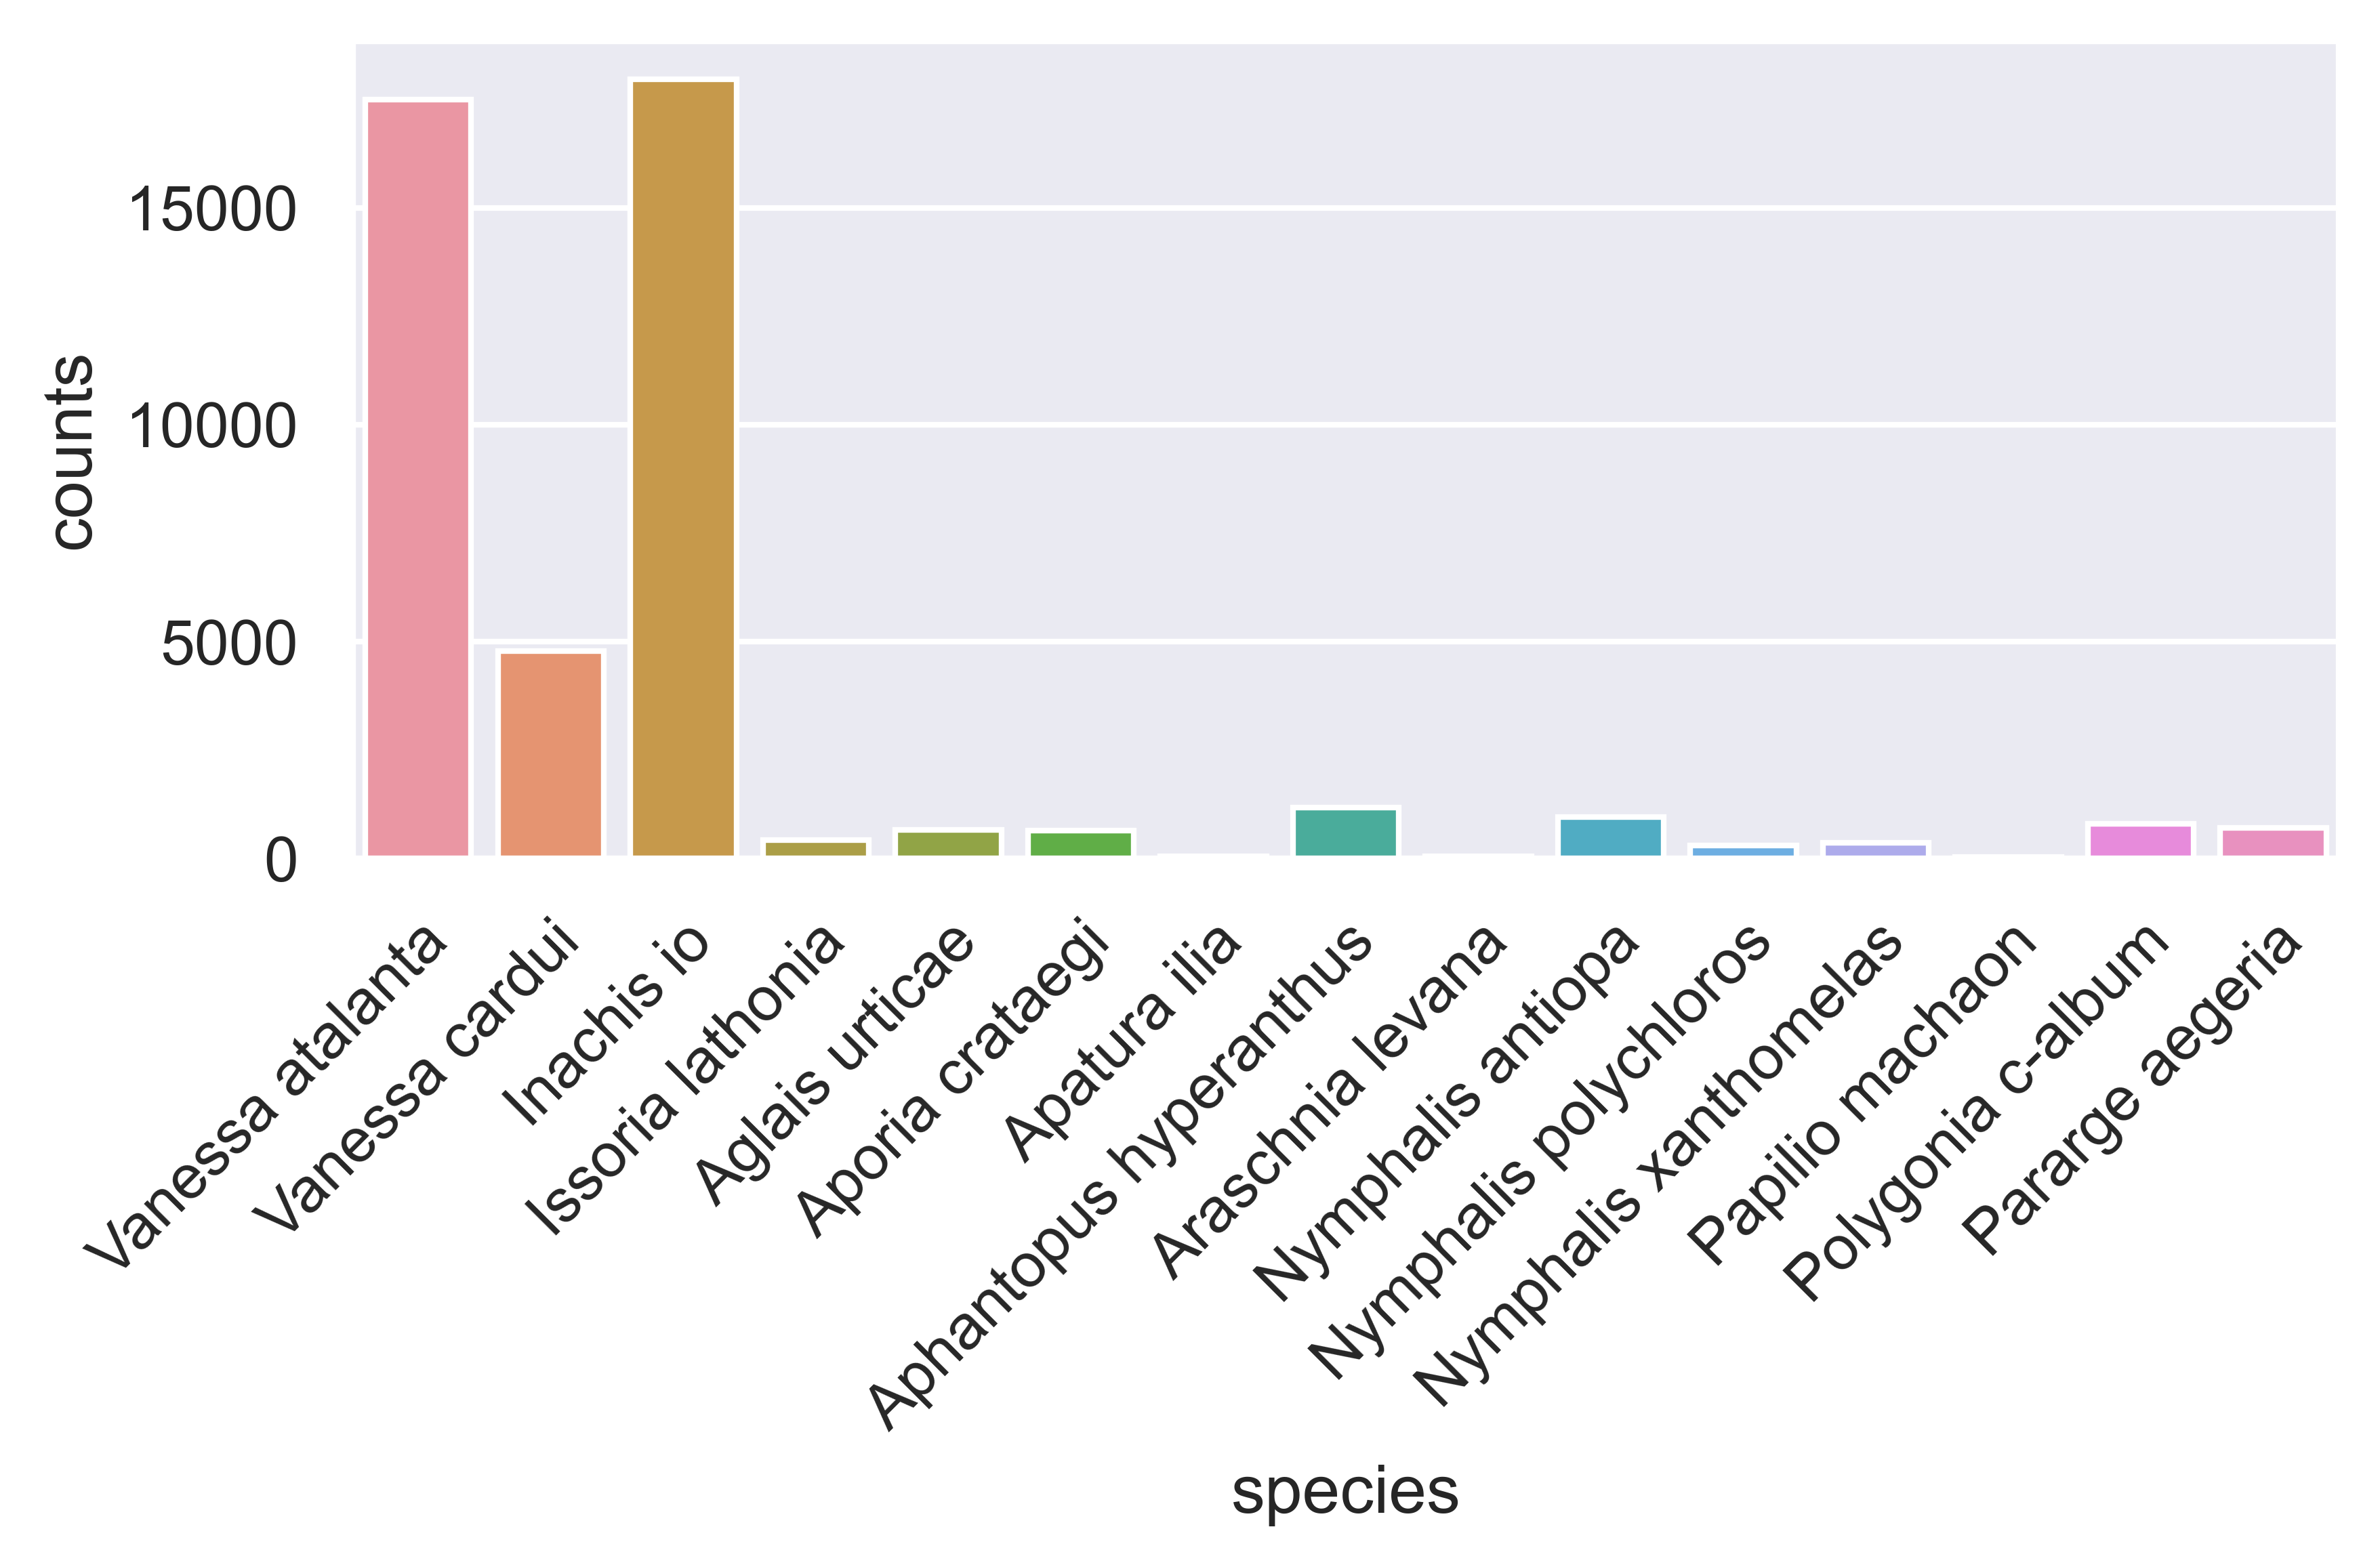
\includegraphics[width=0.9\textwidth]{figs/1-total-count_per_species.png}
			\caption{Total number of observations per species}
			\label{fig:total-count}
		\end{figure}
	\end{frame}

	%%%%%%%%%%%%%%%%%%%%%%%%%%%%%%%%%%%%%%%%%%%%%%%%%%%%%%%%%%%%%%%%
	
	\begin{frame}{Preliminary analysis}
		\begin{figure}
			\centering
			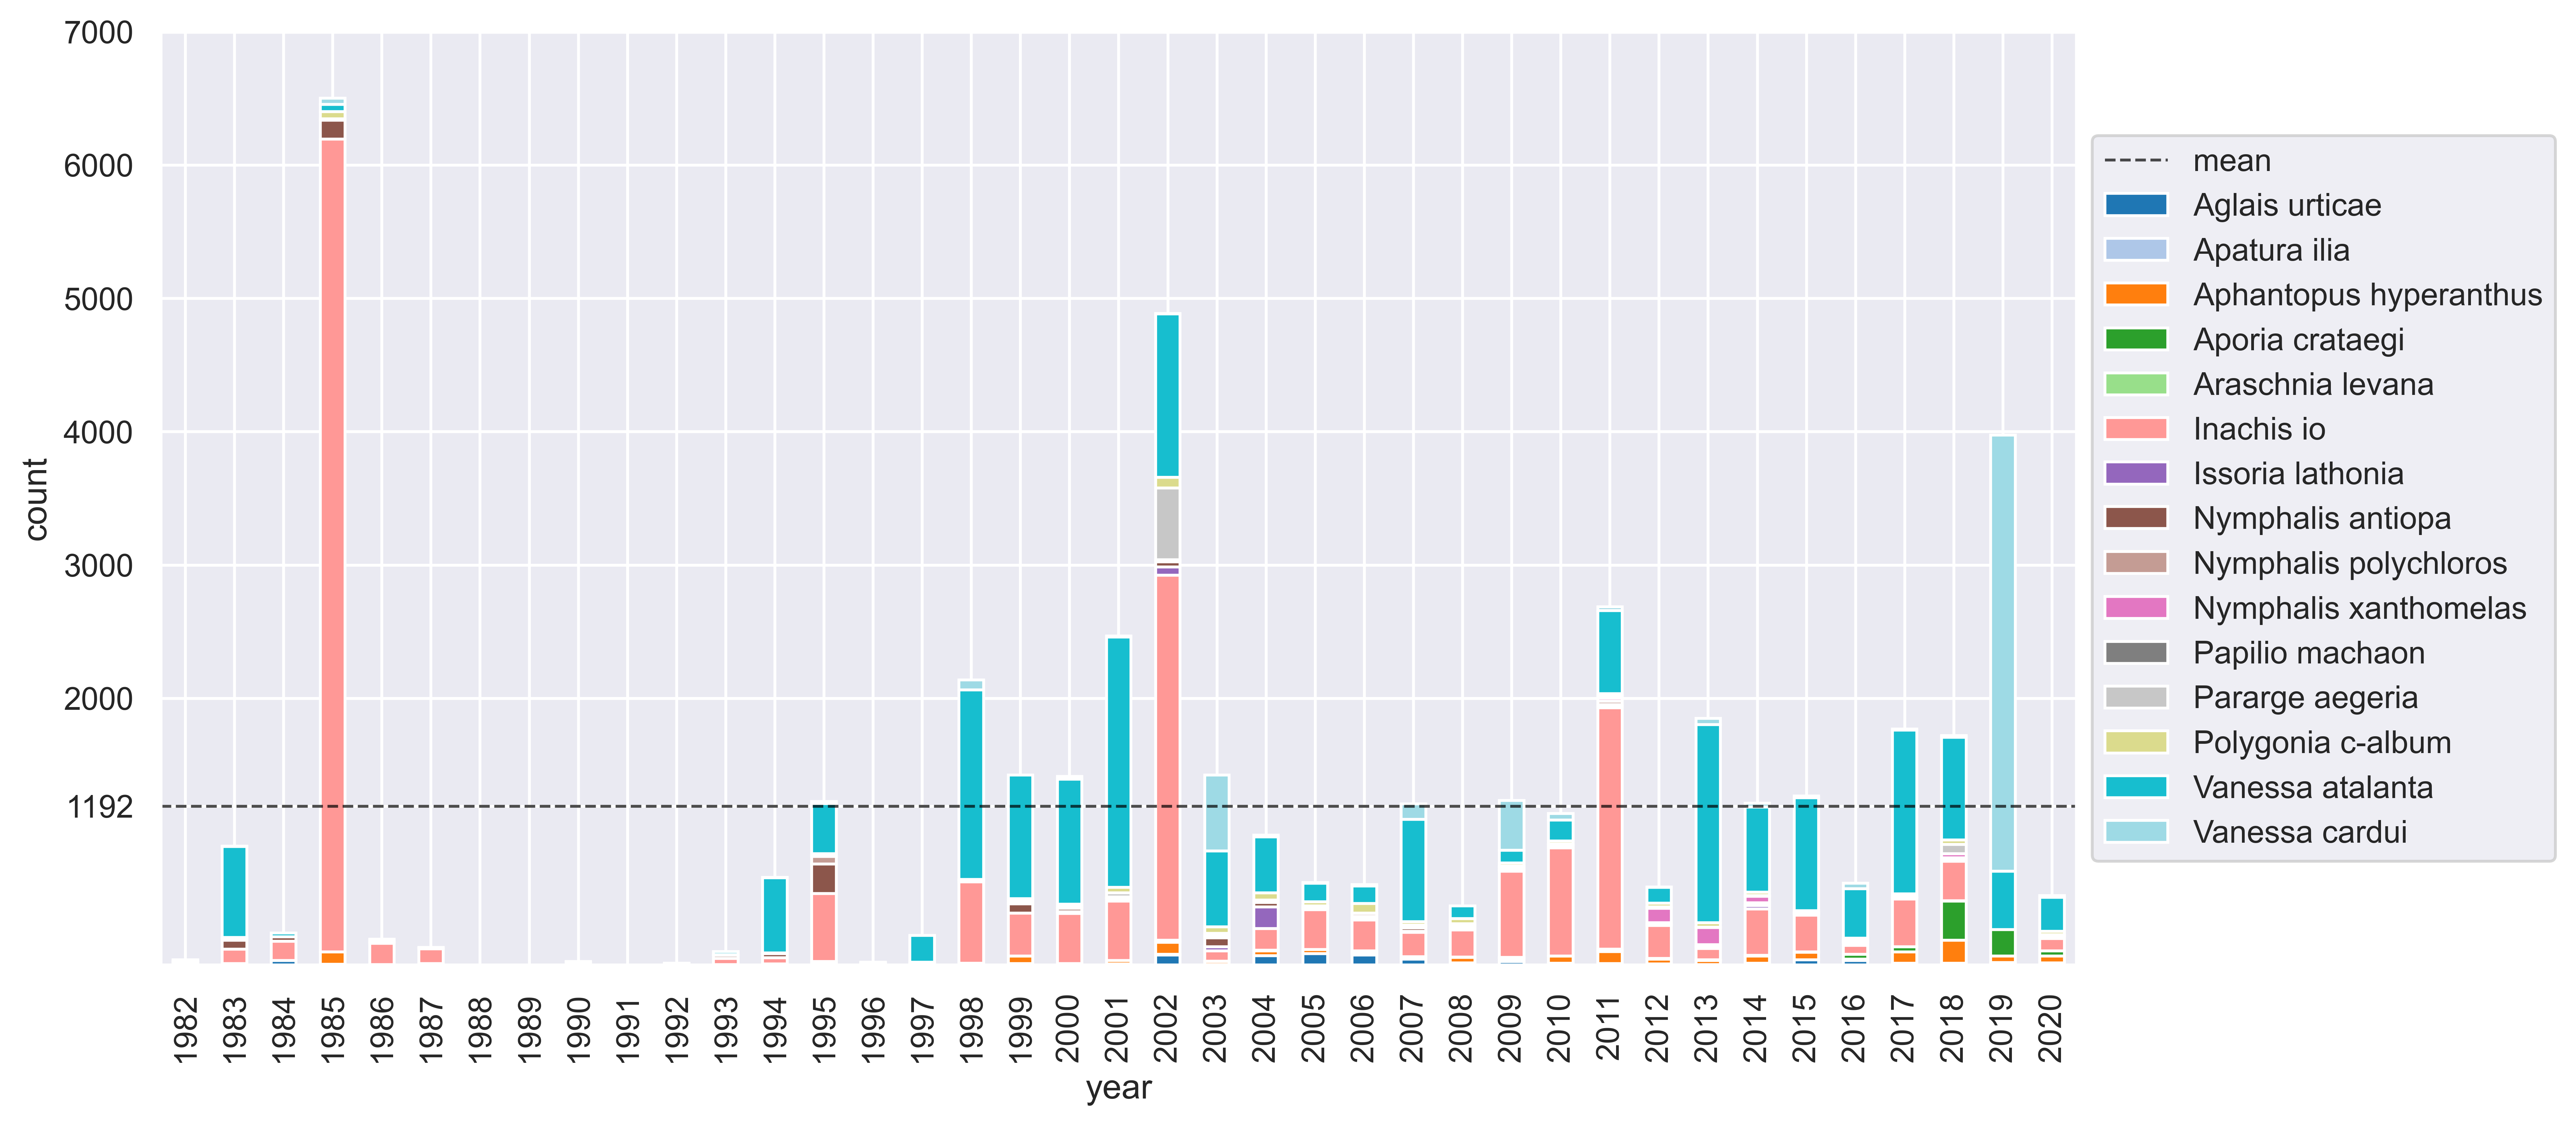
\includegraphics[width=0.9\textwidth]{figs/2-total-count_per_year_per_species.png}
			\caption{Annual butterfly count split into individual species}
			\label{fig:annual-count}
		\end{figure}
	\end{frame}

	%%%%%%%%%%%%%%%%%%%%%%%%%%%%%%%%%%%%%%%%%%%%%%%%%%%%%%%%%%%%%%%%
	
	\begin{frame}{Preliminary analysis}
		\begin{figure}
			\centering
			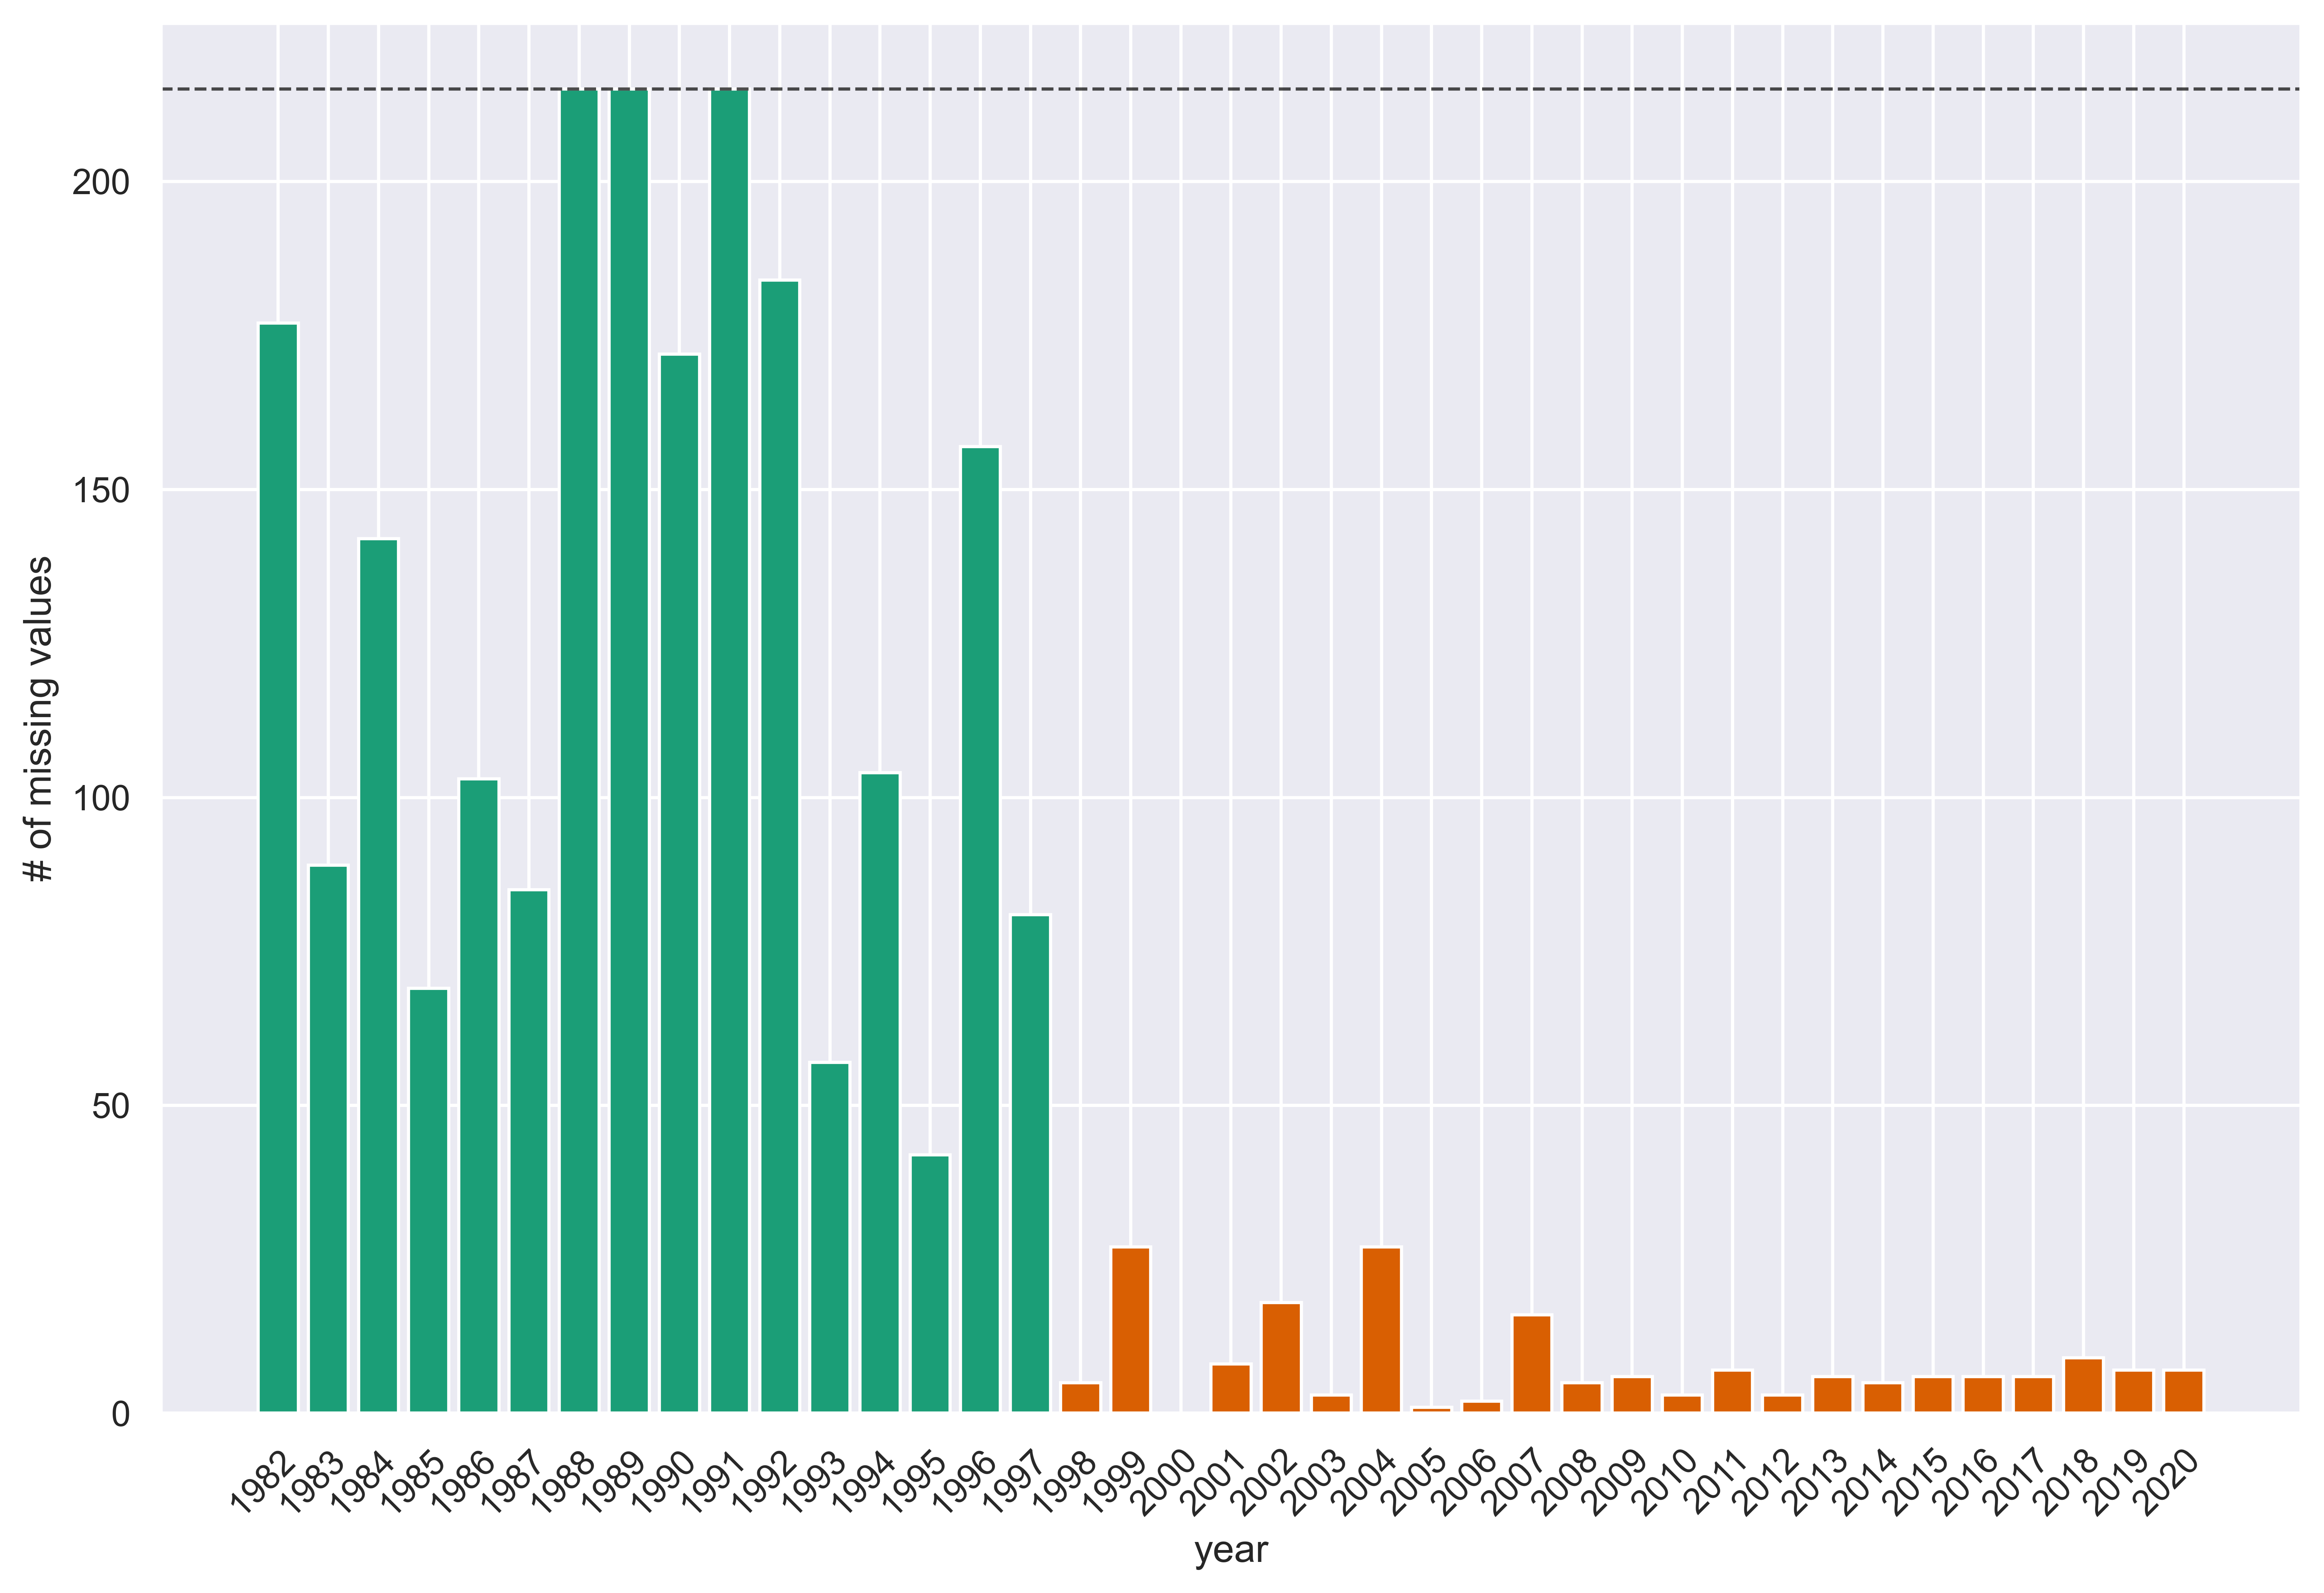
\includegraphics[width=0.9\textwidth]{figs/3-nans_per-year_updated.png}
			\caption{High number of missing values in early records}
			\label{fig:missing-values}
		\end{figure}
	\end{frame}

	%%%%%%%%%%%%%%%%%%%%%%%%%%%%%%%%%%%%%%%%%%%%%%%%%%%%%%%%%%%%%%%%
	
	\begin{frame}{First appearance}
		\begin{columns}
			\column{0.5\textwidth}
			\begin{figure}
				\centering
				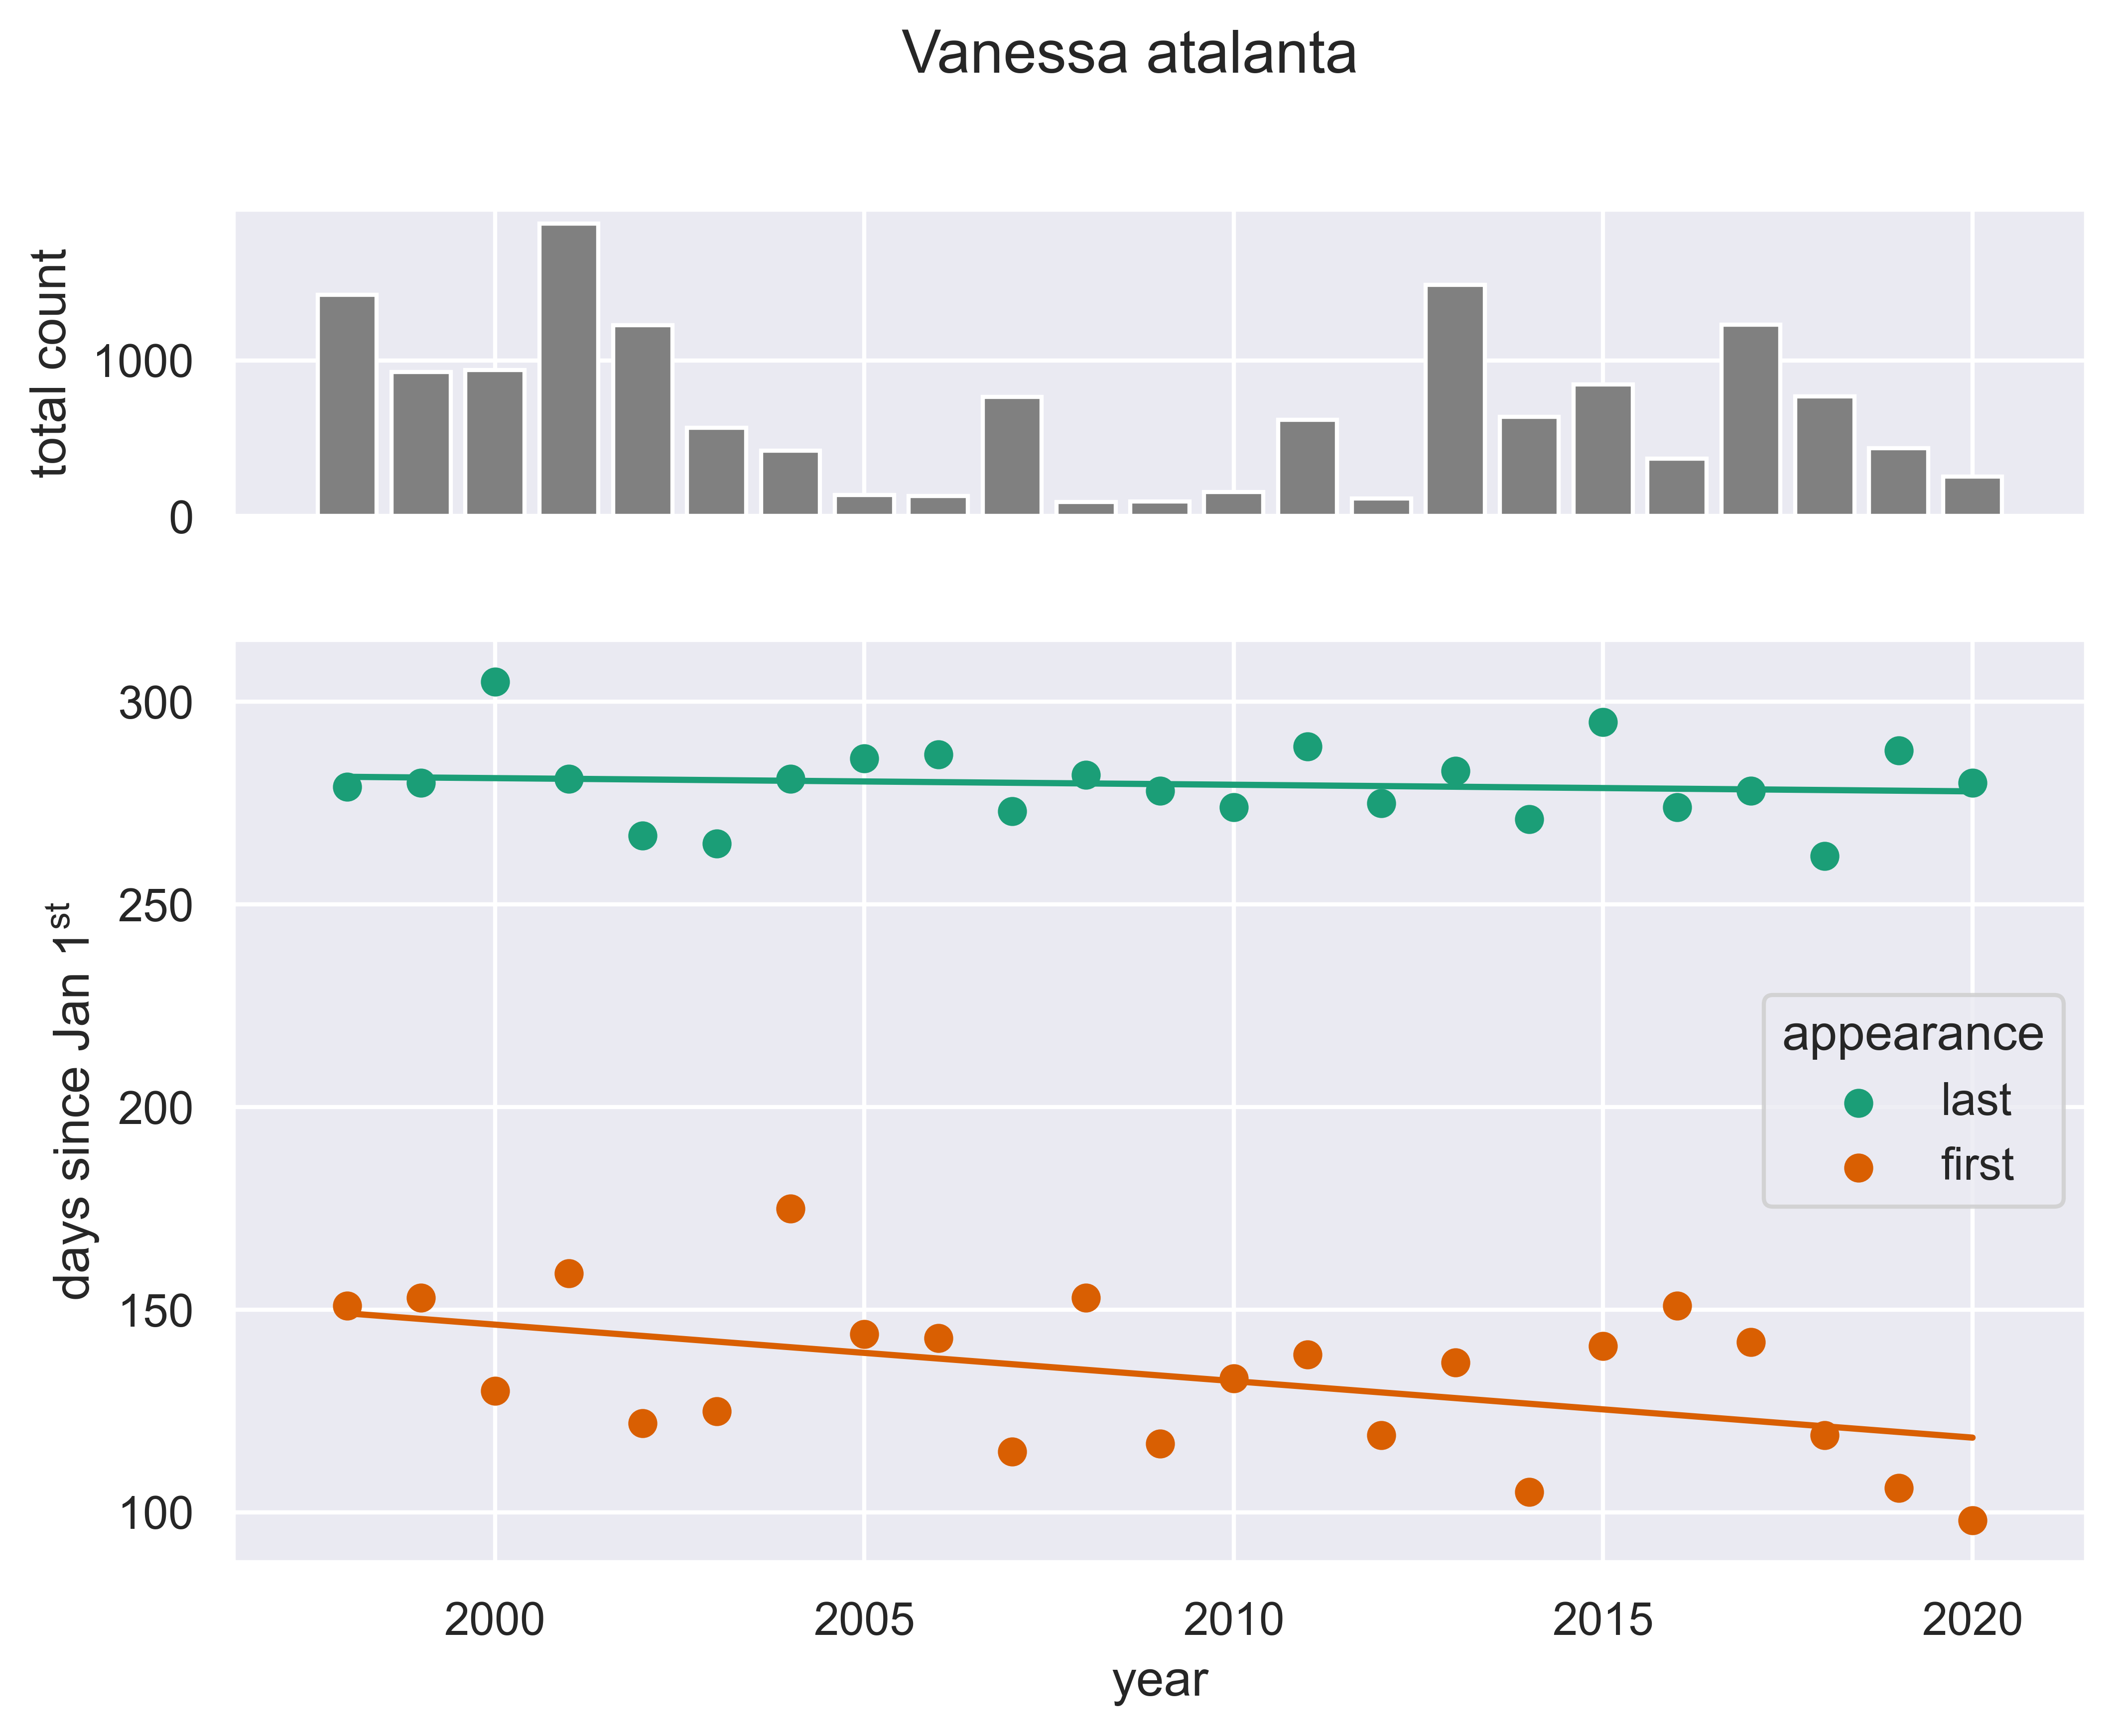
\includegraphics[width=1\textwidth]{figs/4-1-Vanessa atalanta_linregress.png}
				\caption{First annual observation tends to be earlier in recent years.}
				\label{fig:first-app}
			\end{figure}
			\column{0.5\textwidth}
			Significant (\(p < 0.05\)) trend in earlier \textbf{first} appearance:
			\begin{itemize}
				\setlength\itemsep{-0.5em}
				\item \textit{Vanessa atalanta}
				\item \textit{Inachis io}
				\item \textit{Polygonia c-album}
			\end{itemize}
		\end{columns}
	\end{frame}

	%%%%%%%%%%%%%%%%%%%%%%%%%%%%%%%%%%%%%%%%%%%%%%%%%%%%%%%%%%%%%%%%
	
	\begin{frame}{First appearance}
		\begin{columns}
			\column{0.5\textwidth}
			\begin{figure}
				\centering
				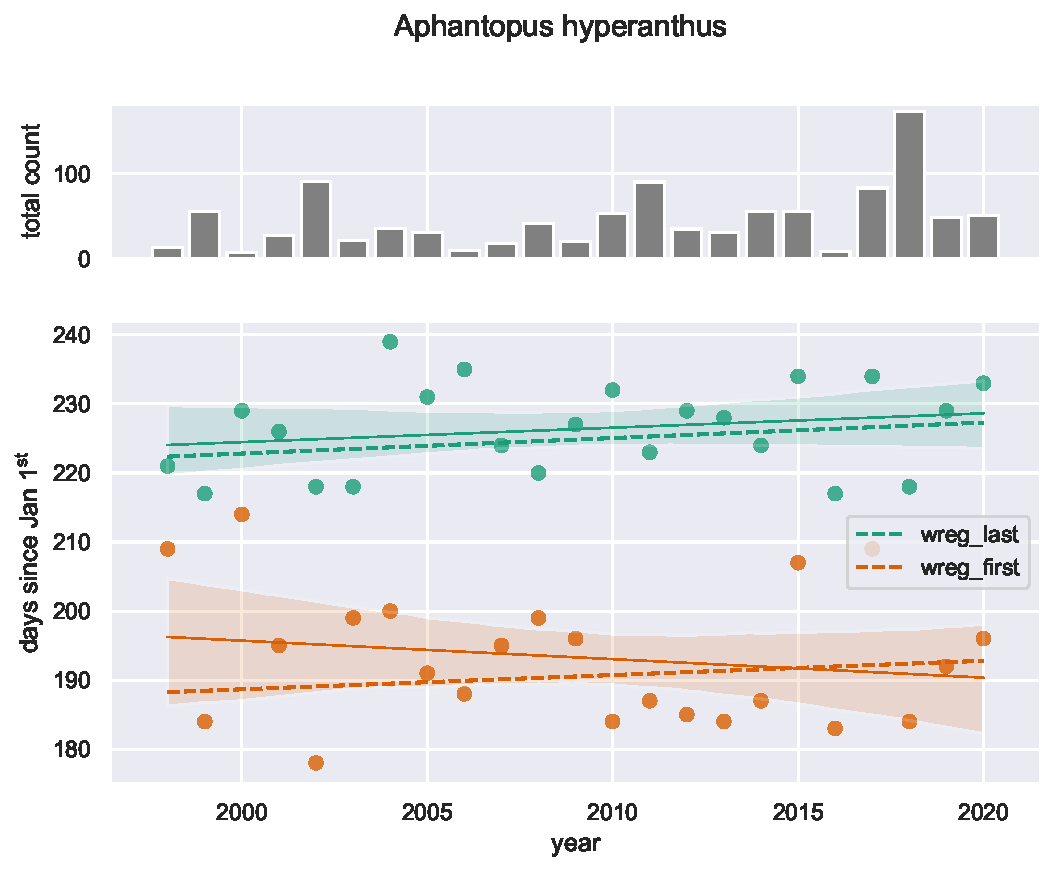
\includegraphics[width=1\textwidth]{figs/4-1-Aphantopus hyperanthus.pdf}
				\caption{Other species show no clear trend in first annual record.}
				\label{fig:first-app-not-sig}
			\end{figure}
			\column{0.5\textwidth}
			No significant (\(p > 0.05\)) trend in earlier \textbf{first} appearance:
			\begin{itemize}
				\setlength\itemsep{-0.5em}
				\item \textit{Vanessa cardui}
				\item \textit{Issoria lathonia}
				\item \textit{Aglais urticae}
				\item \textit{Aporia crataegi}
				\item \textit{Apatura ilia}
				\item \textit{Aphantopus hyperanthus}
				\item \textit{Araschnia levana}
				\item \textit{Nymphalis antiopa}
				\item \textit{Nymphalis polychloros}
				\item \textit{Nymphalis xanthomelas}
				\item \textit{Papilio machaon}
				\item \textit{Pararge aegeria}
			\end{itemize}
		\end{columns}
	\end{frame}

	%%%%%%%%%%%%%%%%%%%%%%%%%%%%%%%%%%%%%%%%%%%%%%%%%%%%%%%%%%%%%%%%
	
	\begin{frame}{Outbreaks}
		\begin{figure}
			\centering
			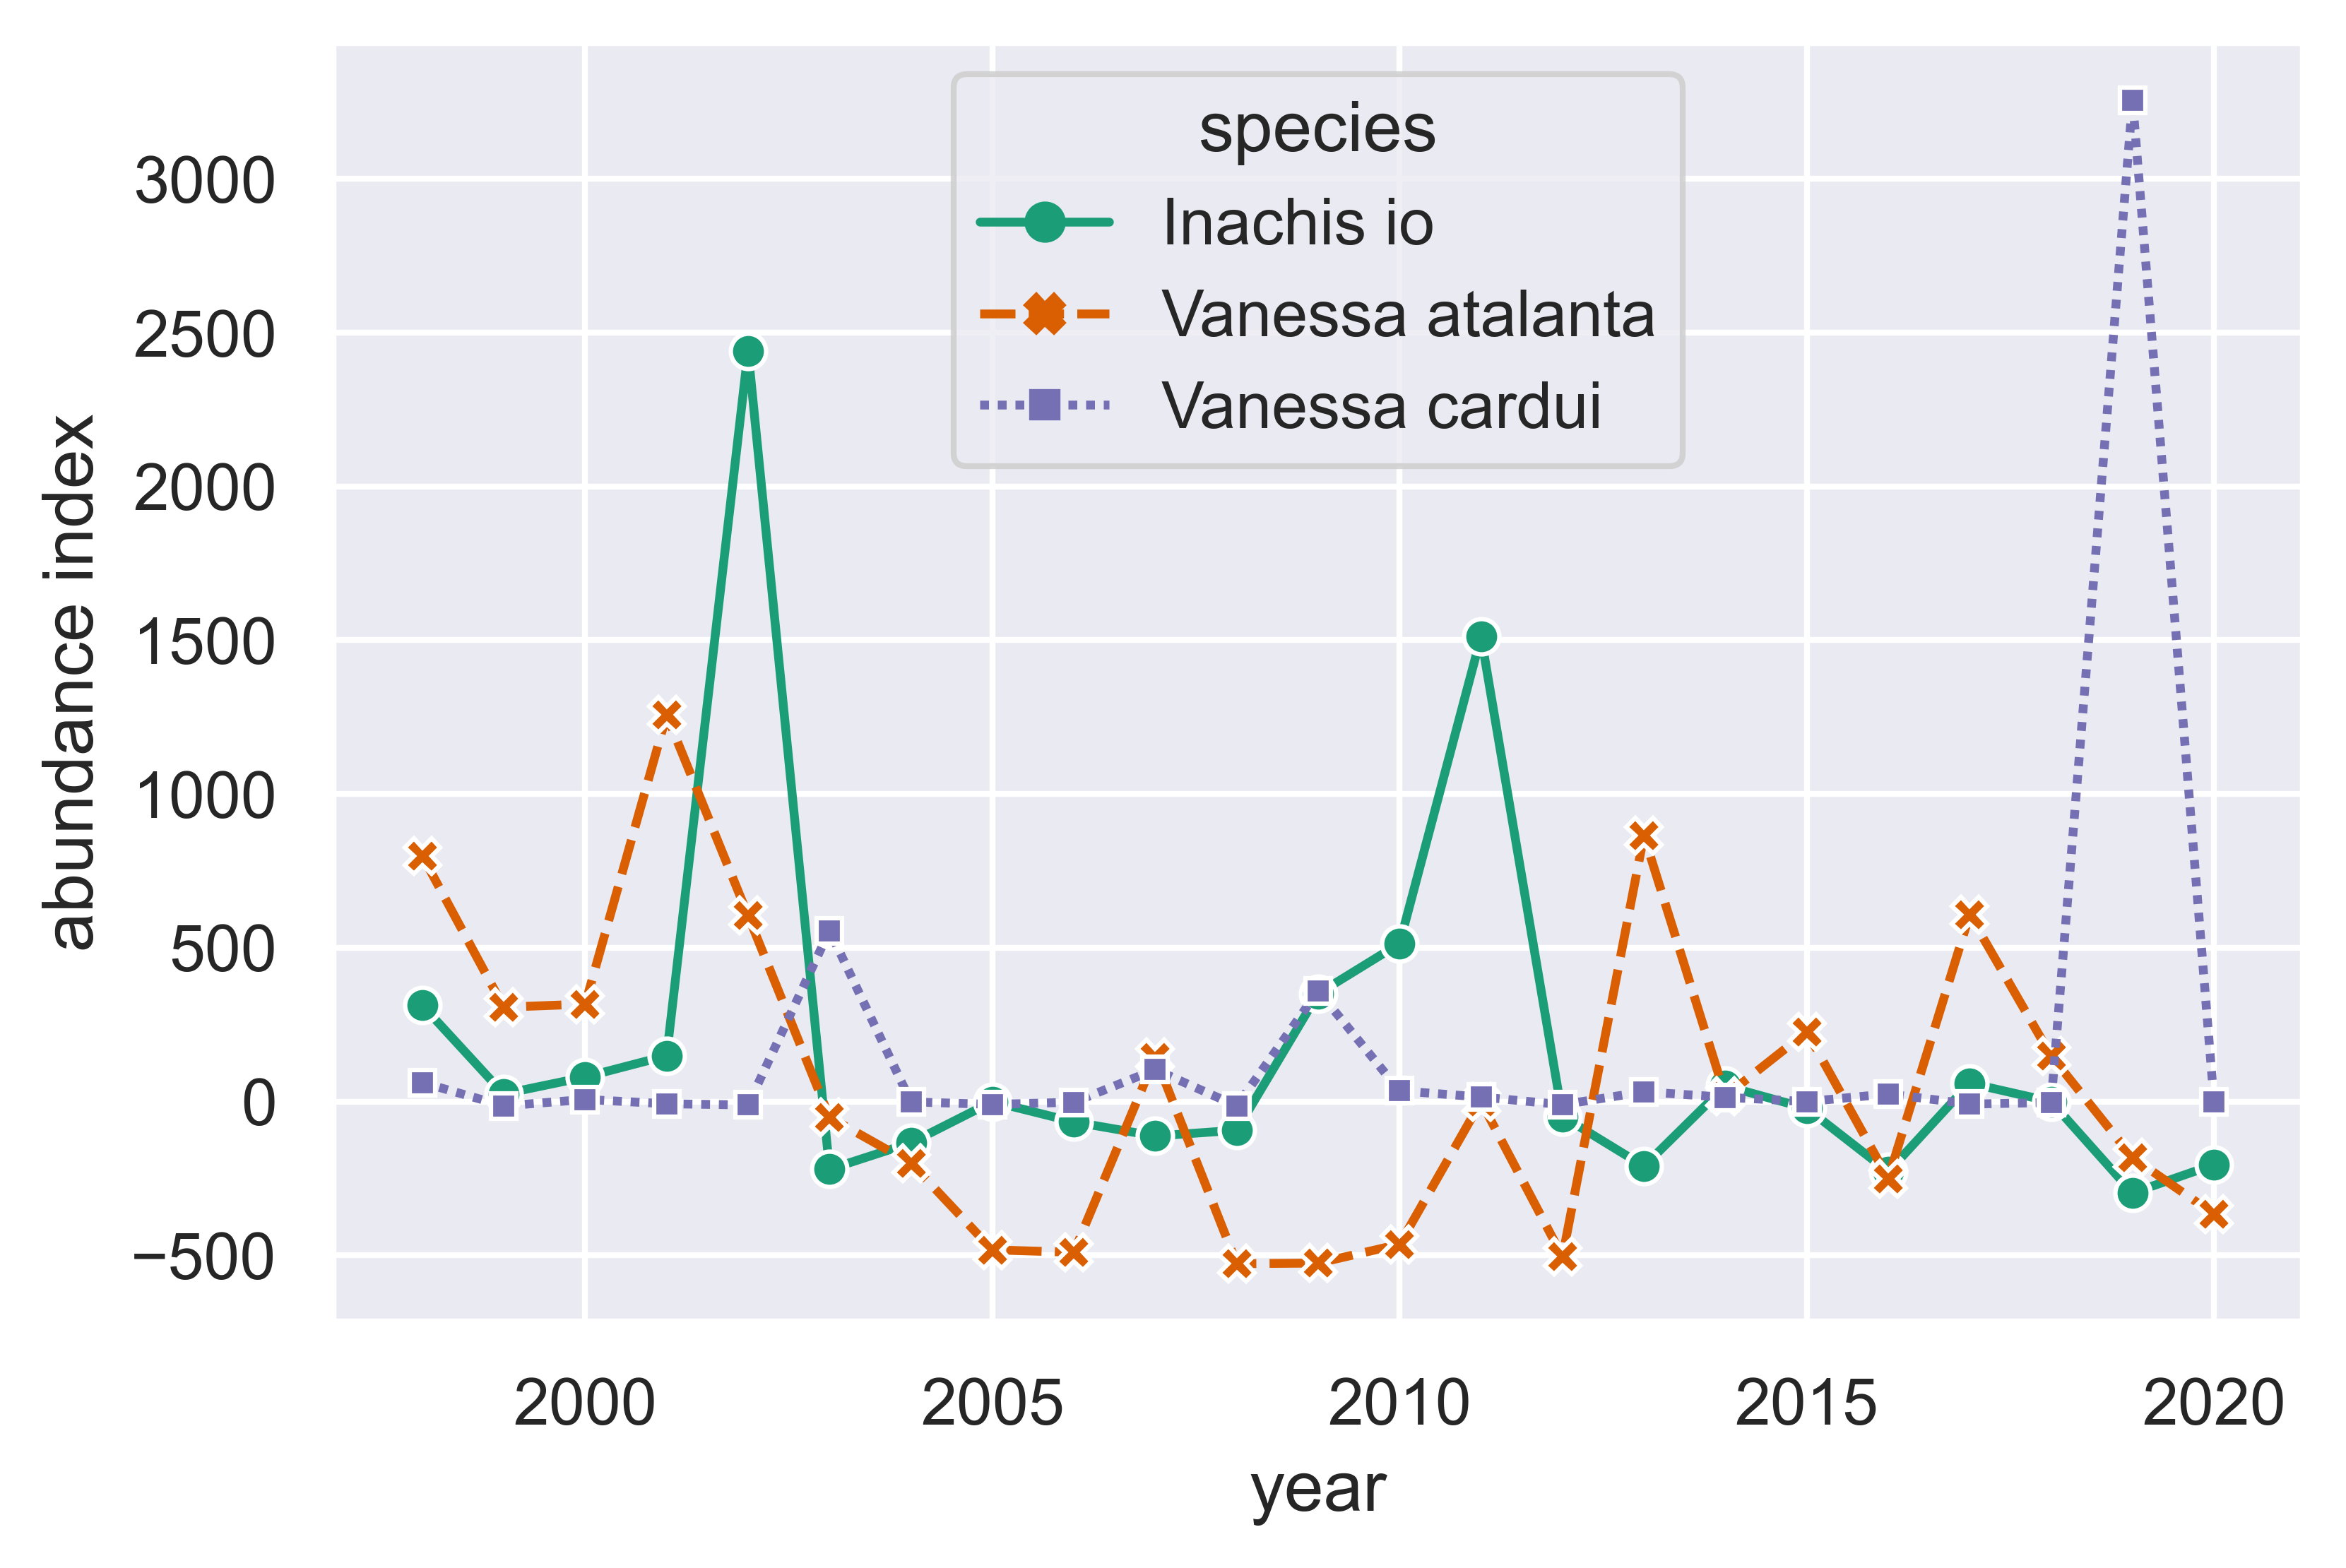
\includegraphics[width=0.9\textwidth]{figs/4-2-outbreaks_per-year.png}
			\caption{Annual number of observations with zero reflecting the \textbf{median} across all years (i.e., \textit{abundance index})}
			\label{fig:outbreaks}
		\end{figure}
	\end{frame}

	%%%%%%%%%%%%%%%%%%%%%%%%%%%%%%%%%%%%%%%%%%%%%%%%%%%%%%%%%%%%%%%%
	
	\begin{frame}{Outbreaks}
		\begin{figure}
			\centering
			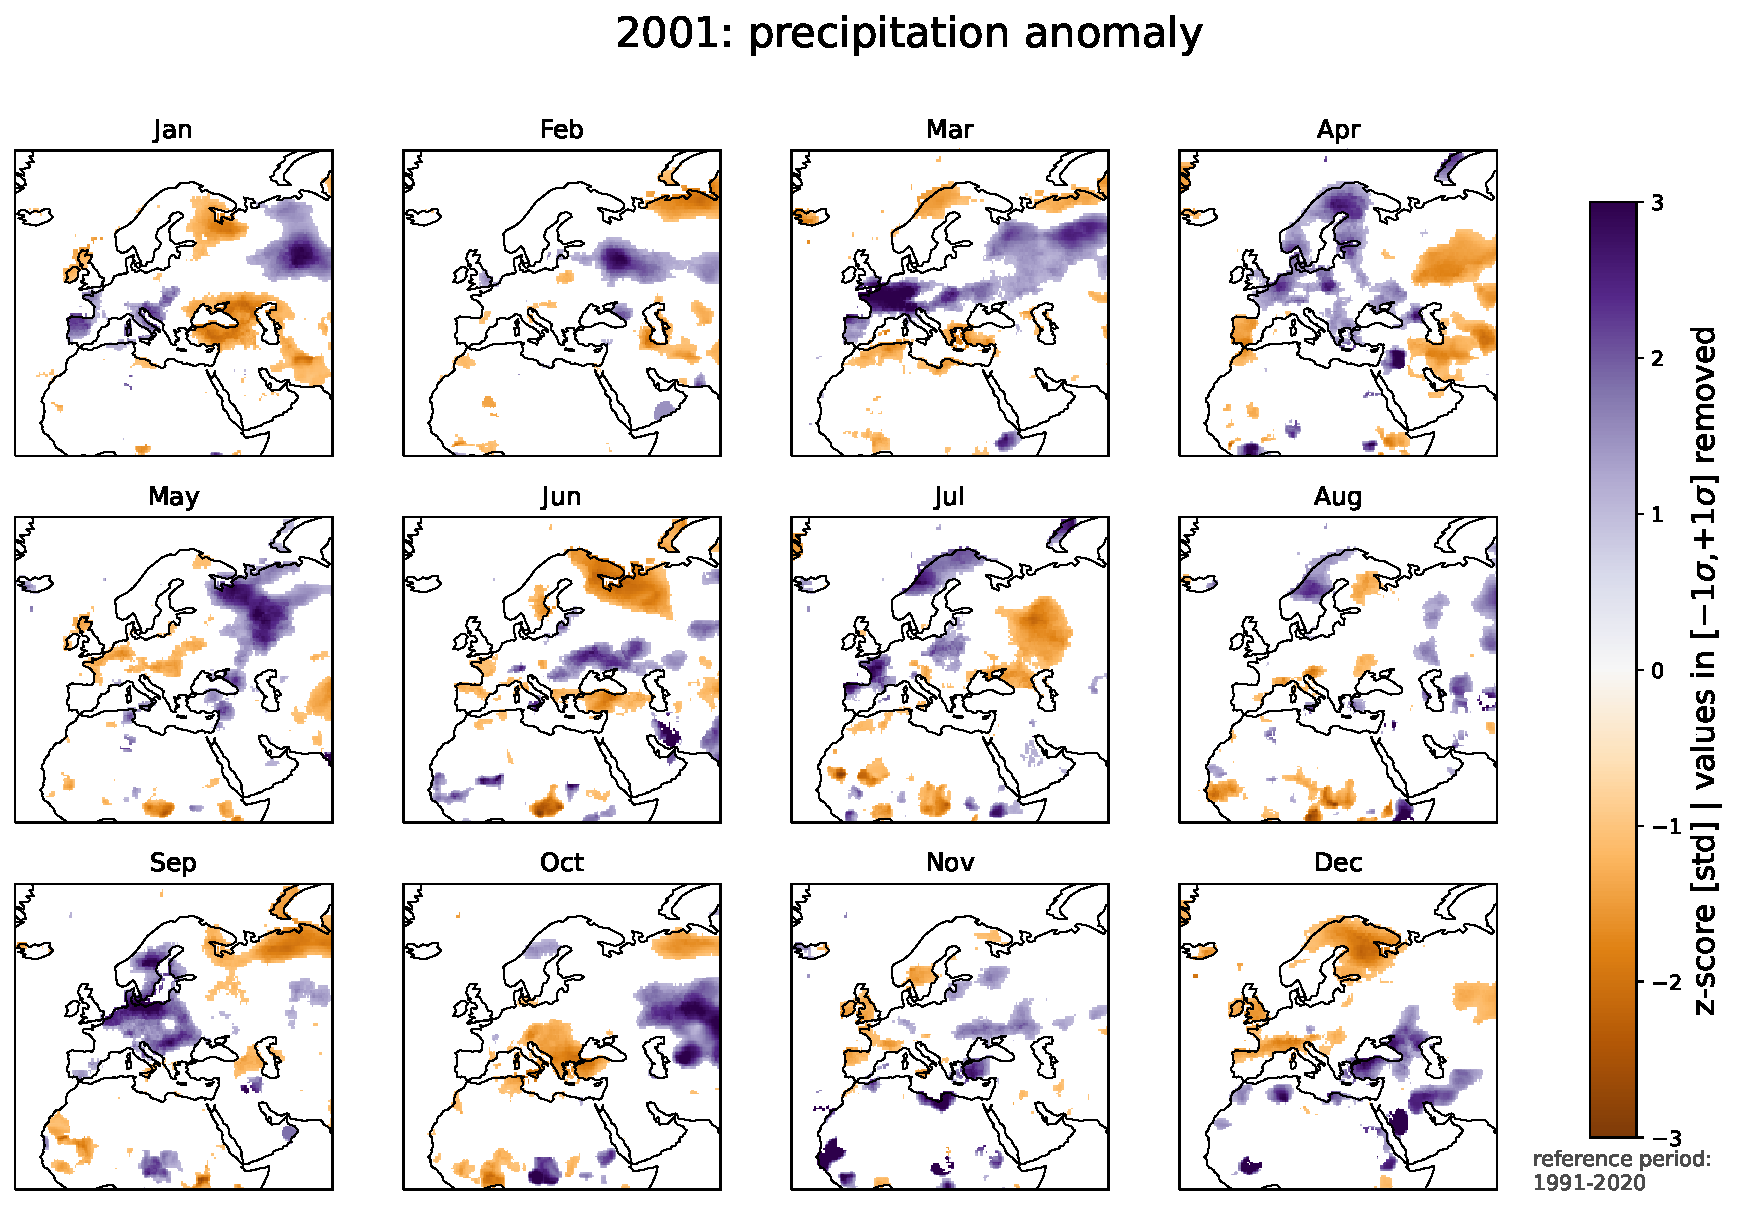
\includegraphics[width=0.9\textwidth]{figs/4-3-precipitation-2001.pdf}
			\caption{Exemplary climate anomaly during year of high \textit{vanessa atalanta} emergence on Courish Spit}
			\label{fig:climate-anomalies}
		\end{figure}
	\end{frame}

	%%%%%%%%%%%%%%%%%%%%%%%%%%%%%%%%%%%%%%%%%%%%%%%%%%%%%%%%%%%%%%%%
	
	\begin{frame}{Outbreaks}
		\begin{figure}
			\centering
			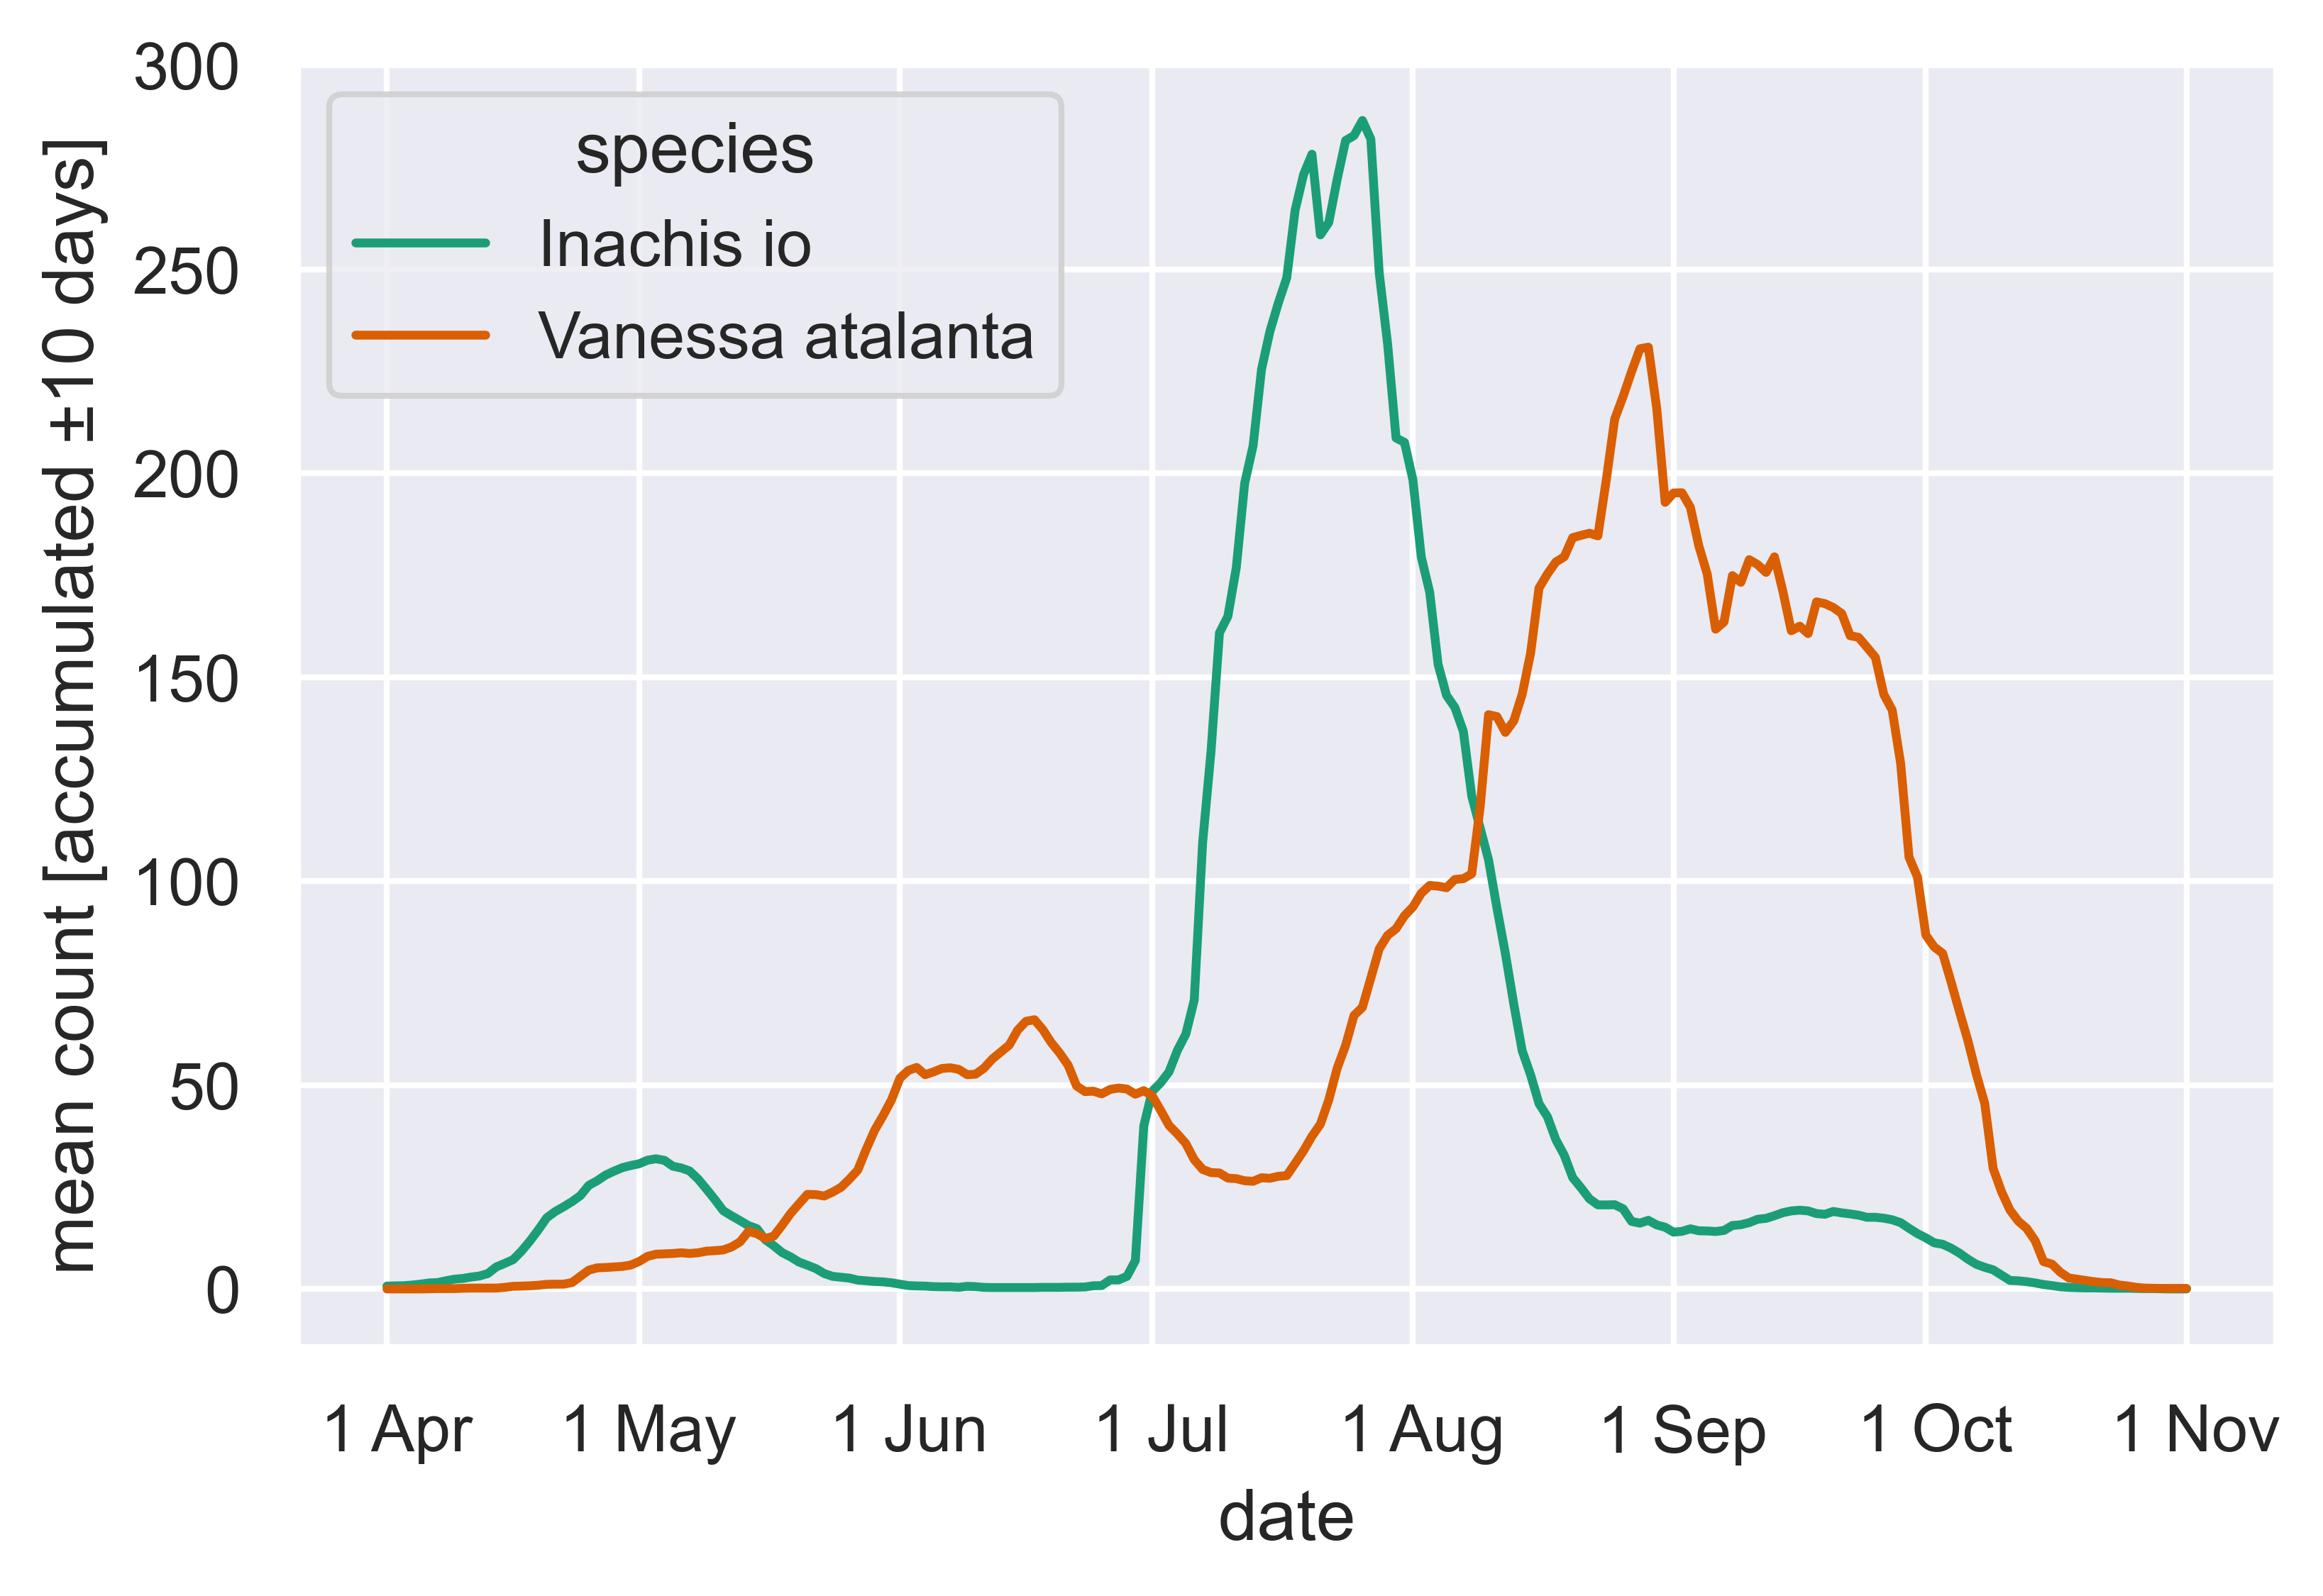
\includegraphics[width=0.9\textwidth]{figs/5-outbreaks_mean-seasonal-pattern.png}
			\caption{Mean seasonal pattern}
			\label{fig:seasonal-pattern}
		\end{figure}
	\end{frame}

	%%%%%%%%%%%%%%%%%%%%%%%%%%%%%%%%%%%%%%%%%%%%%%%%%%%%%%%%%%%%%%%%
	
	\begin{frame}{Outbreaks}
		\begin{figure}
			\centering
			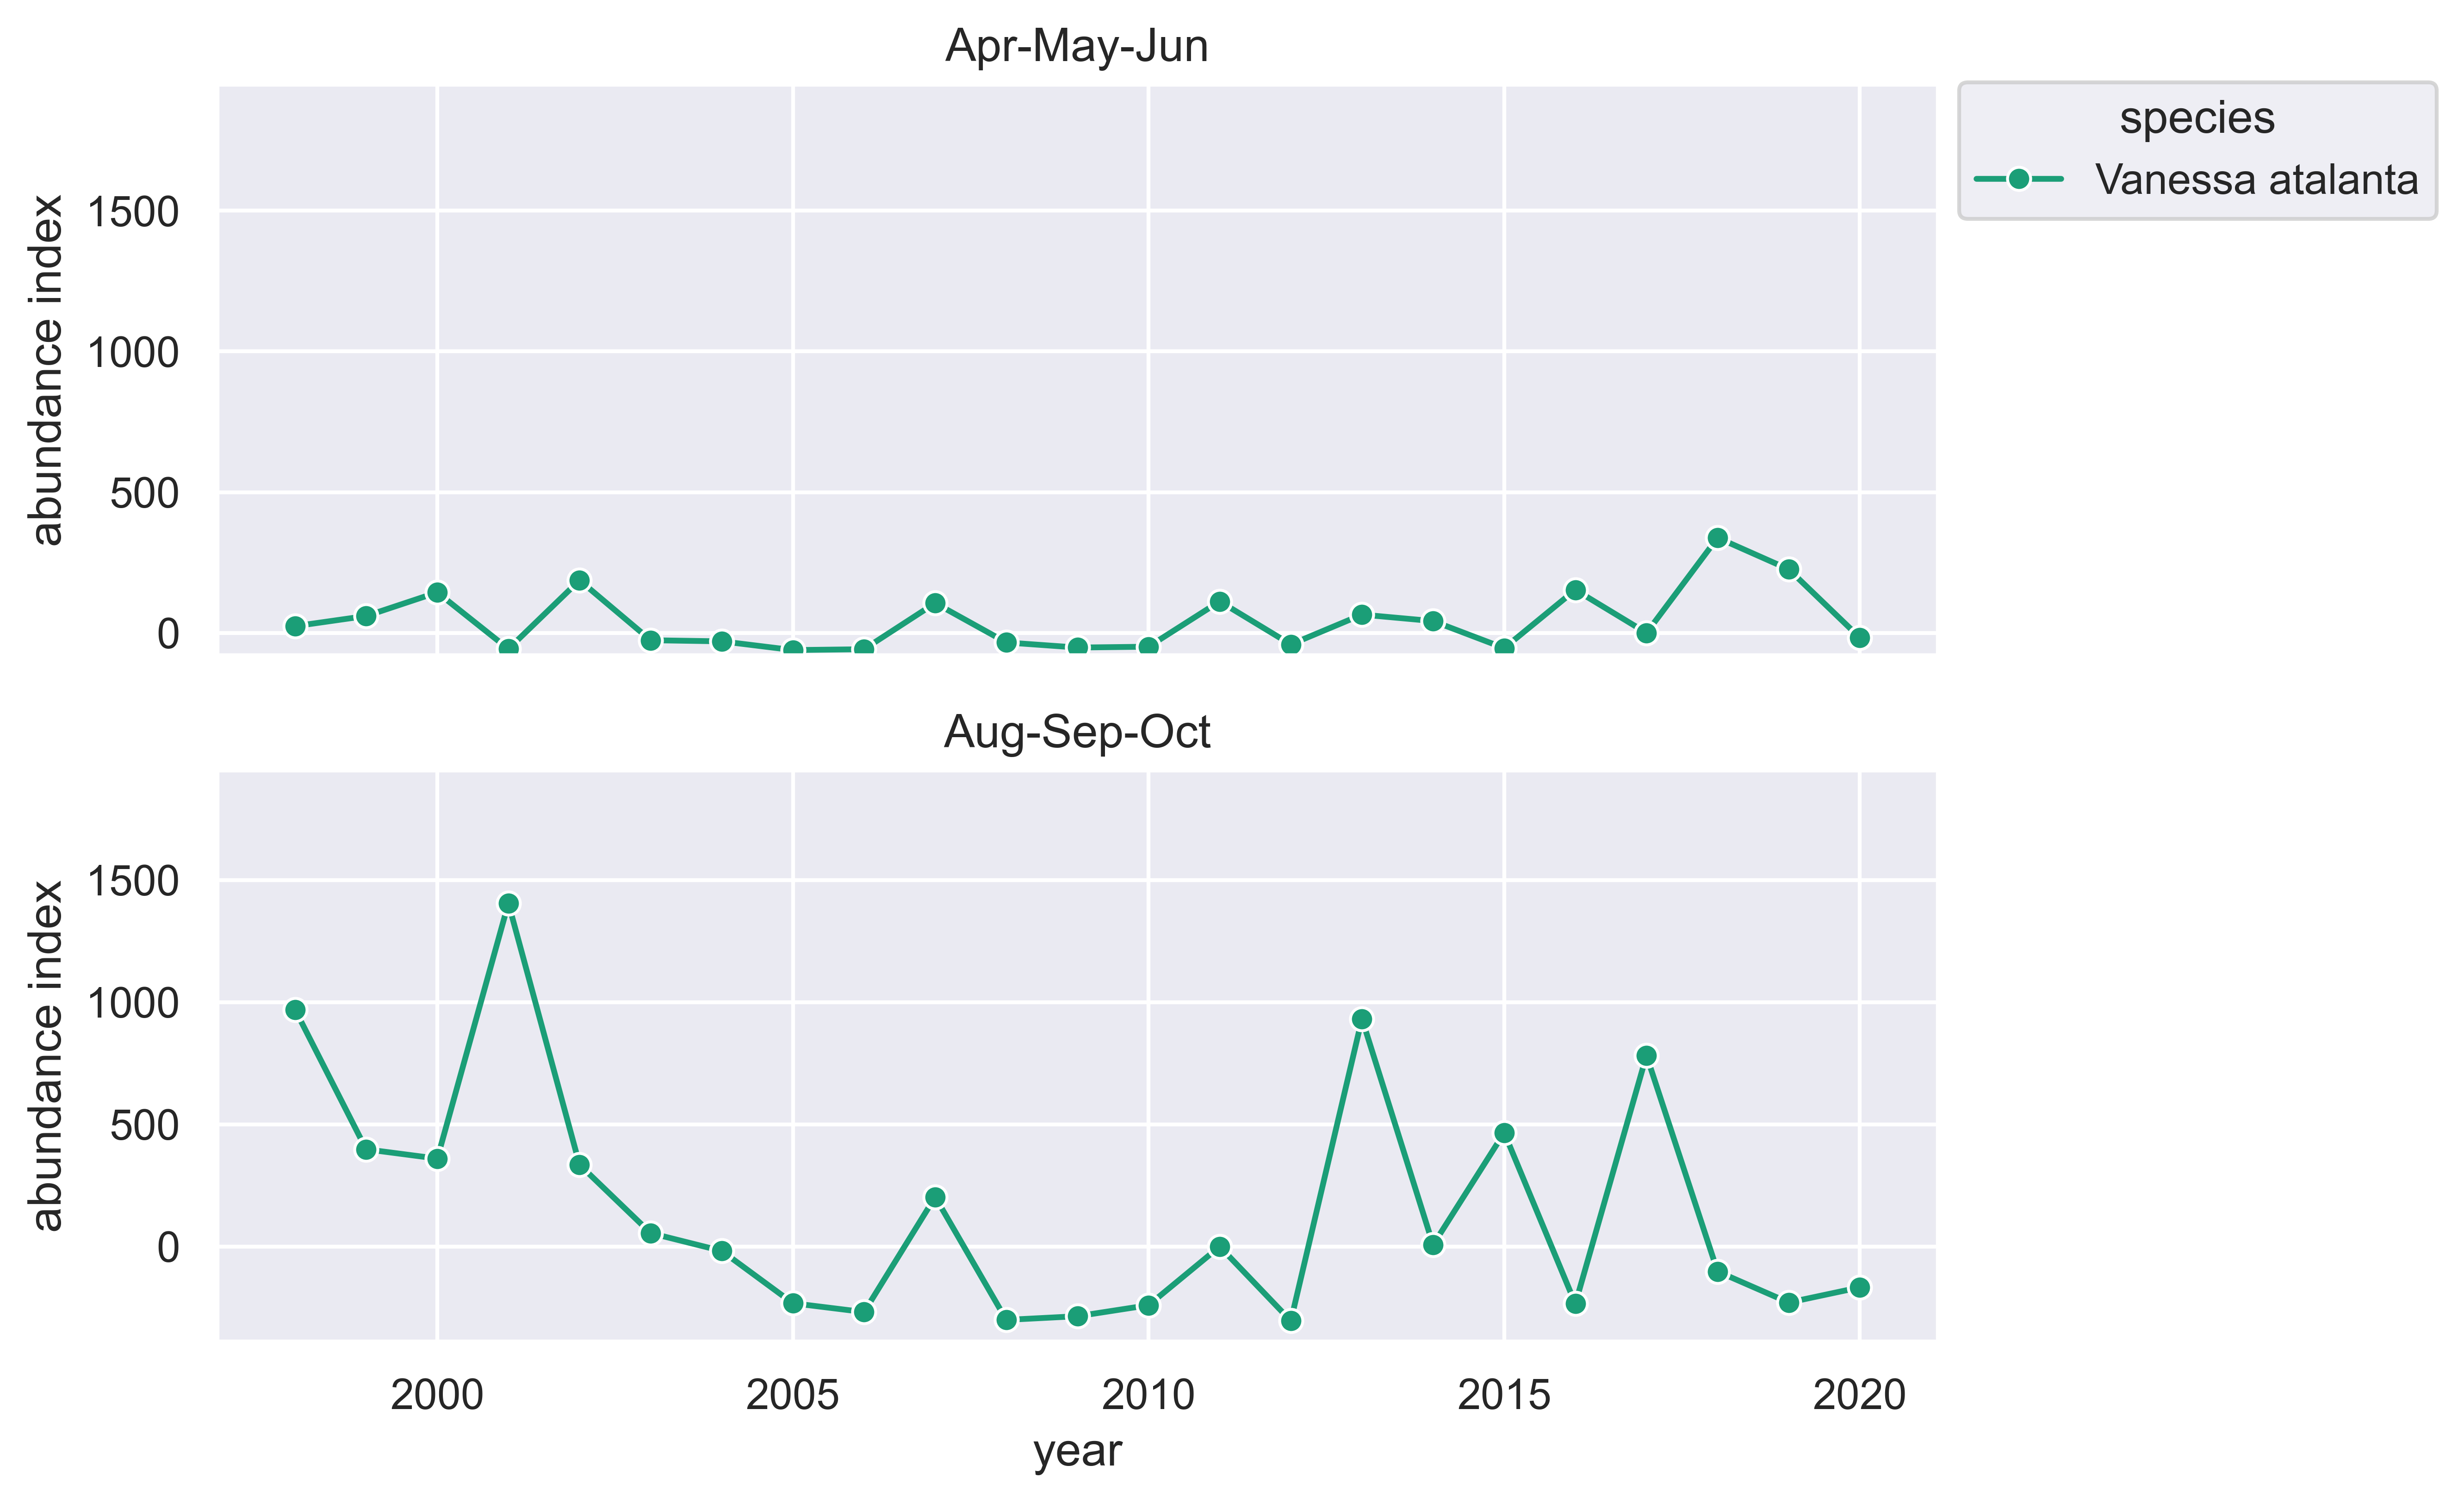
\includegraphics[width=0.9\textwidth]{figs/6-outbreaks_per-season.png}
			\caption{Temporal split of abundance index}
			\label{fig:outbreaks-by-season}
		\end{figure}
	\end{frame}
	
	%%%%%%%%%%%%%%%%%%%%%%%%%%%%%%%%%%%%%%%%%%%%%%%%%%%%%%%%%%%%%%%%
	
	\begin{frame}{Outbreaks}
		\begin{figure}
			\centering
			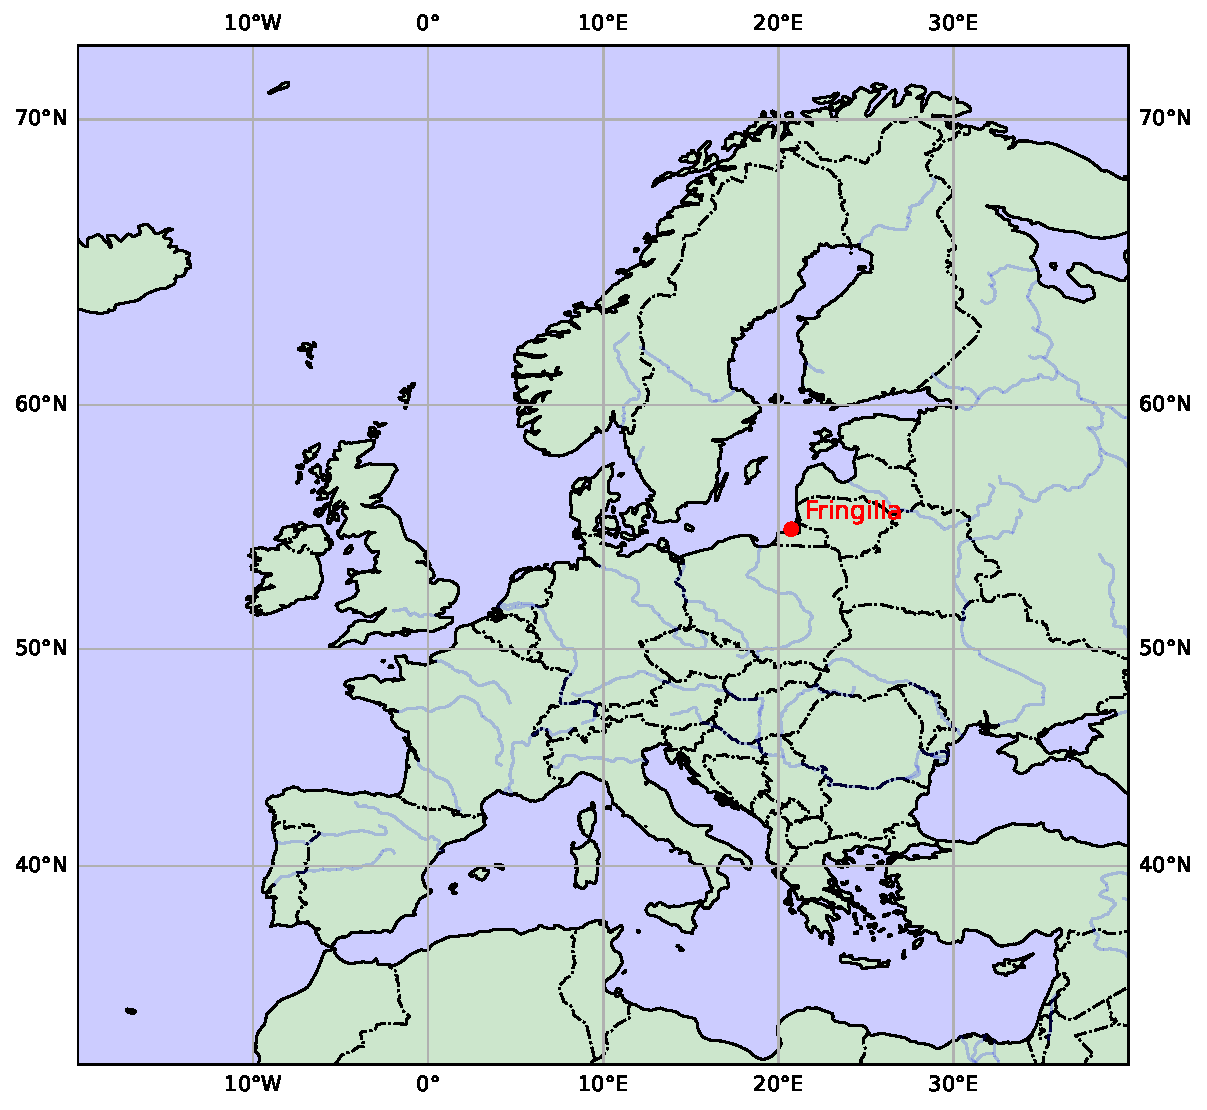
\includegraphics[height=0.8\textheight]{figs/7-map-europe.pdf}
			\caption{Climate anomalies in Northern Europe trigger outbreaks?}
			\label{fig:map-europe}
		\end{figure}
	\end{frame}
	
	%%%%%%%%%%%%%%%%%%%%%%%%%%%%%%%%%%%%%%%%%%%%%%%%%%%%%%%%%%%%%%%%
	
	\begin{frame}[allowframebreaks]
		\printbibliography
	\end{frame}
	
	\maketitle
	
\end{document}